\section{Zielsetzung}
Im Versuch sollen durch das Verfahren des optischen Pumpens die Energieaufspaltungen
in der Hyperfeinstruktur oder der Zeeman-Aufspaltung mit hoher Präzision gemessen werden.
Konkret werden die Energieaufspaltungen zweier Rubidium-Isotope ermittelt.

\section{Theorie}
Während die Besetzung der innersten Elektronenschalen nach dem Pauliprinzip vollständig besetzt
wird, so erfolgt die Besetzung der äußeren Schalen temperaturabhängig.
Für die zwei Zustände mit den Energien $W_1$ und $W_2$ und den Besetzungszahlen $N_1$ und
$N_2$ gilt demnach folgendes Verhältnis zwischen den Besetzungszahlen:
\begin{align*}
    \frac{N_{2}}{N_{1}} = \frac{g_{2}}{g_{1}}\frac{\exp(-W_{2}/\text{kT})}{\exp(-W_{1}/\text{kT})} \; .
\end{align*}
Die Größen $g_{\text{i}}$ geben hierbei die Anzahl der zu den Energien $W_1$ und $W_2$ gehörenden
Zustände an.
Mittels des Verfahrens des optischen Pumpens ist es möglich, dieses Verhältnis zu verändern
oder gar zu invertieren ($N_{2} > N_{1}$).
Zunächst soll im Folgenden betrachtet werden, wie sich die Energieniveaus eines Atoms aufspalten können.

\subsection{Energieaufspaltung}
In einer ersten Näherung soll zunächst der Fall betrachtet werden, in dem davon ausgegangen wird, der
Kernspin verschwindend ist.
Der Gesamtdrehimpuls der Valenzelektronen des Atoms $\vec{\text{J}}$ erzeugt hierbei
ein magnetisches Moment $\vec{\mu}_{\text{J}}$, welche in folgendem Zusammenhang stehen:
\begin{align*}
    \vec{\mu}_{\text{J}} &= -\text{g}_{\text{J}} \cdot \mu_{\text{B}} \cdot \vec{\text{J}} \\
    |\vec{\mu}_{\text{J}}| &= \hspace{1em} \text{g}_{\text{J}} \cdot \mu_{\text{B}} \cdot \sqrt{ \text{J} (\text{J}+1) }
\end{align*}
Hier beschreibt $\mu_{\text{B}}$ das Bohr'sche Magneton.
Der Landé-Faktor $\text{g}_{\text{J}}$ dient zur Berücksichtigung des Umstandes, dass sich der Gesamtdrehimpuls aus dem Bahndrehimpuls $\vec{\text{L}}$ und dem Spin $\vec{\text{S}}$ des Valenzelektrons zusammensetzt.
Für die magnetischen Momente, die durch Spin und Bahndrehimpuls hervorgerufen werden $\vec{\mu}_{\text{L,S}}$, gilt:
\begin{align*}
    |\vec{\mu}_{\text{L}}| &= \mu_{\text{B}} \sqrt{\text{L} (\text{L}+1)} \\
    |\vec{\mu}_{\text{S}}| &= \text{g}_{\text{S}} \cdot \mu_{\text{B}} \sqrt{\text{S}(\text{S}+1)} \; .
\end{align*}
Vektoriell beschrieben, sieht die Kopplung der magnetischen Momente, die aus dem Spin und dem Bahndrehimpuls resultieren wie folgt aus:
\begin{align*}
    \vec{\mu}_{\text{J}} &= \vec{\mu}_{\text{L}} + \vec{\mu}_{\text{S}} \\
    |\vec{\mu}_{\text{J}}| &= |\vec{\mu}_{\text{L}}| \cos(\beta) + |\vec{\mu}_{\text{S}}| \cos{\alpha} \; .
\end{align*}
Nun lässt sich mit Hilfe des Cosinussatzes, angewendet auf das Dreieck, das von $\vec{\mu}_{\text{L}}, \vec{\mu}_{\text{J}} \text{und} \vec{\mu}_{\text{S}}$ aufgesapnnt wird, eine Formel zur Berechnung des Landé-Faktors herleiten:
\begin{align}
    \text{g}_{\text{J}} = \frac{(\text{g}_{\text{s}} + 1) \cdot \text{J} (\text{J} + 1) + (\text{g}_{\text{s}}-1) \cdot \left[\text{S}
    \cdot (\text{S}+1) - \text{L} (\text{L} + 1) \right]}{2 \cdot \text{J} (\text{J} +1 )}
    \label{eq:La-Fa.gj}
\end{align}
Durch Anlage eines äußeren Magnetfeldes B, kommt es nun zur Aufspaltung der Energieniveaus, was als Zeeman-Effekt bekannt ist. Die Energie der magnetischen Wechselwirkung wird wie folgt beschrieben:
\begin{align}
    E_{\text{mag}} &= \vec{\mu}_{\text{J}} \cdot \vec{\text{B}} \\
    &= \text{M}_\text{J} \cdot \text{g}_\text{J} \cdot \mu_{\text{B}} \cdot \text{B} \; .
    \label{eq:E_mag}
\end{align}
Hierbei gilt für die Orientierungsquantenzahl $\text{M}_\text{J}$ auf Grund der Richtungsquantelung: $\text{M}_{\text{J}} \in [-\text{J}, -\text{J}+1,\hdots,\text{J}-1,\text{J}]$ .

\noindent Nun sollen die fälle betrachtet werden, in denen der Kernspin nicht verschwindet.
Bei hinreichend schwachem Magnetfeld, wovon im Falle des Versuches ausgegangen werden kann, koppeln der Gesamtdrehimpuls der Elektronenhülle $\vec{\text{J}}$ und der Kernspin $\vec{text{I}}$ vektoriell aneinander zu einem Gesamtdrehimpuls des Systems $\vec{\text{F}}$:
\begin{align*}
    \vec{\text{F}} = \vec{\text{I}} + \vec{\text{J}} \; .
\end{align*}
Durch den nicht mehr verschwindenden Kernspin, spalten sich die Energieniveaus nun in die Hyperfeinstruktur auf.
Die Anzahl der Niveaus wird durch $2\text{J}+1$ oder $2\text{I}+1$ ermittelt, je nachdem, ob J größer als I ist oder anders herum.
Die Quantenzahl F beschreibt dabei, wie sich die einzelnen Niveaus aufspalten und läuft von I+J bis $|\text{I}-\text{J}|$.
Die Hyperfeinstruktur kann wiederum in $2\text{F}+1$ Zeeman-Niveaus aufgespalten werden, indem ein äußeres Magnetfeld angelegt wird.
Eine Beispielhafte Aufspaltung ist in Abbild \ref{abb:Aufspaltung} zu sehen.
\FloatBarrier
\begin{figure}
    \centering
    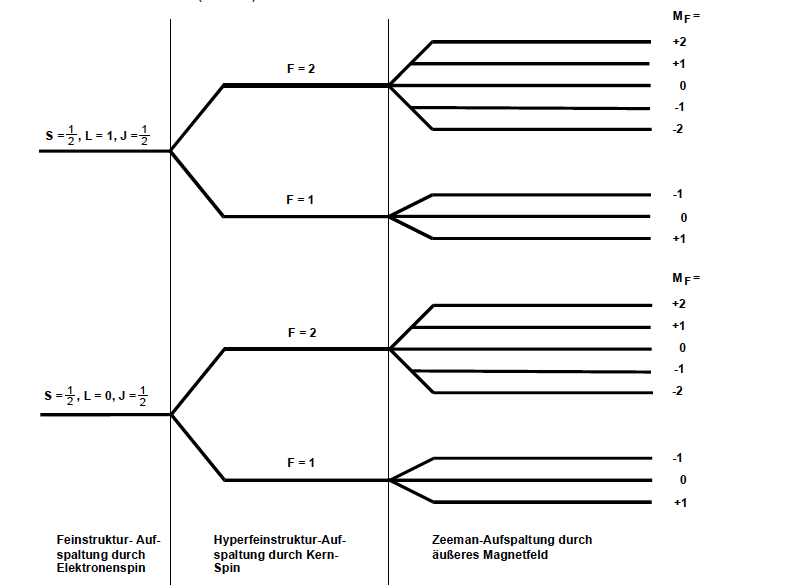
\includegraphics[width=0.7\textwidth]{Aufspaltung.PNG}
    \caption{Aufspaltung der Energieniveaus eines Alkaliatoms mit I = $\frac{3}{2}$ und J = $\frac{1}{2}$ auf Grund von Elektronenspin, Kernspin und externem Magnetfeld. \cite{Q1}}
    \label{abb:Aufspaltung}
\end{figure}
\FloatBarrier
Zwischen zwei benachbarten Energieniveaus herrscht eine Energiedifferenz, die wie folgt berechnet werden kann:
\begin{align*}
    E_{\text{HF}} = \text{g}_{\text{F}} \mu_{\text{B}} \text{B} \; .
\end{align*}
Mittels vektorieller Betrachtung lässt sich der Landé-Faktor für die Zeeman-Aufspaltung bestimmen:
\begin{align*}
    |\vec{\mu}_{\text{F}}| &= \text{g}_{\text{F}} \cdot \mu_{\text{B}} \sqrt{\text{F} (\text{F}+1)} \\
    &=\text{g}_{\text{J}} \cdot \mu_{\text{B}} \sqrt{\text{J} (\text{J} + 1)} \cdot \cos\left(\measuredangle(\vec{\text{J}},\vec{\text{F}})\right) +
    \text{g}_{\text{I}} \cdot \mu_{\text{K}} \sqrt{ \text{I}(\text{I}+1) } \cdot \cos\left(\measuredangle(\vec{\text{I}},\vec{\text{F}})\right) \; .
\end{align*}
Hierbei beschreibt $\mu_{\text{K}}$ das magnetische Moment des Kerns und $\text{g}_{\text{I}}$ den zugehörigen Landé-Faktor.
Allerdings ist auf Grund der großen Massendifferenz zwischen Elektron und Nukleon ( $\rightarrow \mu_{\text{K}} \ll \mu_{\text{B}} $ ) zu beachten, dass in obiger Gleichung der zweite Summand zumeist vernachlässigt wird, womit für den Landé-Faktor folgendes gilt:
\begin{align}
    \text{g}_{\text{F}} \approx \text{g}_{\text{J}} \frac{\text{F} (\text{F} + 1)+\text{J} (\text{J} + 1) - \text{I}(\text{I} + 1)}{2\text{F}(\text{F}+1)} \; .
	\label{eq:La-Fa.gf}
\end{align}

\subsection{Optisches Pumpen}
Wie bereits erwähnt, kann die Besetzung höherer Energieniveaus mit Hilfe der Boltzmannstatistik beschrieben werden.
Mit Hilfe des Verfahrens des optischen Pumpens ist es möglich diese Verteilung zu invertieren, also eine größere Bestzung eines höheren Energiezustandes zu erzeugen.
Um von einem Atom absorbiert zu werden, benötigt ein Photon folgende Energie:
\begin{align*}
    hf = W_{2} - W_{1}
\end{align*}
Diese Energie entspricht der Energie des Photons, was bei einem Übergang von $W_{2}$ auf $W_{1}$ frei würde.
Zunächst soll der Einfachheit halber ein Alkaliatom betrachtet werden, da dies lediglich ein Valenzelektron und keinen Kernspin besitzt.
Der Grundzustand dieses Atoms ist dann ${}^2S_{{}^1\!/\!_2}$ und die ersten beiden angeregten Zustände sind dann ${}^2P_{{}^1\!/\!_2}$ und ${}^2S_{{}^3\!/\!_2}$. Wie in Abbildung \ref{abb:Aufspaltung2} zu sehen, sind zwei Übergänge möglich: $D_{1}$ und $ D_{2} $.
Der Gesamtspin J der Zustände ${}^2S_{{}^1\!/\!_2}$ und ${}^2P_{{}^1\!/\!_2}$ beträgt $\text{J}= {}^1\!/\!_2$. Daraus ergeben sich für die Orientierungsquantenzahl $\text{M}_\text{J}$ folgende mögliche Werte für die Aufspaltung und für die Differenz $\Delta \text{M}_\text{J}$:
\begin{align*}
    \text{M}_\text{J} &= \pm \frac{1}{2} \\
    \Delta \text{M}_\text{J} &= 0, \pm 1 \; .
\end{align*}
\FloatBarrier
\begin{figure}
    \centering
    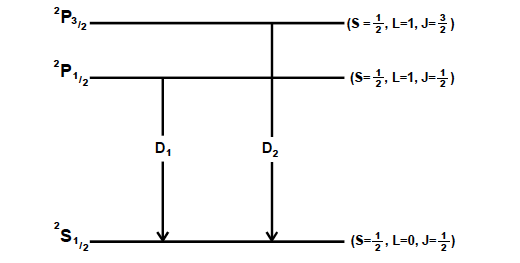
\includegraphics[width= 0.49\textwidth, height=0.3\textwidth]{Aufspaltung2.PNG}
    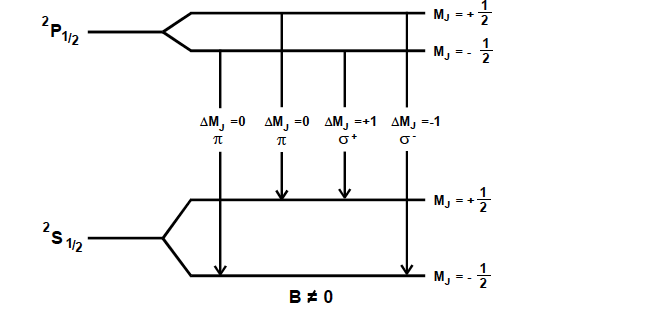
\includegraphics[width=0.40\textwidth, height=0.3\textwidth]{Aufspaltung3.PNG}
    \caption{Dublettstruktur des Alkali-Atoms mit zugehörigen Quantenzahlen, sowie die Zeeman-Aufspaltung des Grundniveaus und des ersten angeregten Zustands mit möglichen Übergängen. \cite{Q1}}
    \label{abb:Aufspaltung2}
\end{figure}
Je nach dem, welcher Übergang stattfindet, ist das dabei emittierte Licht unterschiedlich polarisiert.
Beim $\sigma^+$-Übergang ( $\Delta \text{M} = +1$ ) ist der Spin der emittierten Lichtquanten antiparallel zur Ausbreitungsrichtung und es entsteht rechts zirkular-polarisiertes Licht. Beim $\sigma^-$-Übergang ( $\Delta \text{M} = -1$ ) hingegen sind Spin und Ausbreitungsrichtung parallel. Die beiden $\sigma$-Übergänge werden entlang des Magnetfeldes emittiert, wohingegen der $\pi$-Übergang ( $\Delta \text{M} = +0$ ) senkrecht zum Magnetfeld abgestrahlt wird, wo das Intensitätsmaximum auftreten, und linear polarisiertes Licht emittiert wird.
Nun besteht die Möglichkeit ein Gas aus diesem hypotetischen Alkali-Atom, das sich im thermischen Gleichgewicht befindet,
mit zirkular polarisiertem Licht ($D_1$-Licht) anzuregen und ein äußeres Magnetfeld anzulegen. Da die Orientierungsquantenzahl M hierbei nur +1 oder -1 betragen kann, sind nur Übergänge von ${}^2S_{^1\!/\!_2}$ mit  $M_J=-^1\!/\!_2$ nach ${}^2P_{^1\!/\!_2}$, $M_J=+^1\!/\!_2$ möglich.
Der Übergang vom ersten angeregten Zustand ${}^2P_{^1\!/\!_2}$ mit $M_J=+^1\!/\!_2$ zurück in den Grundzustand findet hierbei durch spontane
Emission statt. Dabei wird sowohl der Grundzustand mit $M_J=-^1\!/\!_2$
als auch der mit $M_J=+^1\!/\!_2$ besetzt. Diese beiden Vorgänge sorgen dafür, dass der energetisch niedrigere Zustand entgegen der thermischen Verteilung ohne Anregung und Magnetfeld, immer weniger besetzt ist und sozusagen "leer" gepumpt wird.
Je weniger der energetisch niedrigere Zustand besetzt ist, umso weniger Lichtquanten werden hier dann absorbiert und das anregende $D_1$-Licht
kann vollständig mit einem Photoddetektor gemessen werden. Die gemessene
Transmission nähert sich asymptotisch dem Wert 1, der nur erreicht werden kann, falls es gelingt, den niedrigeren Zustand mit $M_J=-^1\!/\!_2$ völlig leer zu pumpen.

\subsection{Resonanzstellen}
In Abhängigkeit vom angelegten Magnetfeld existieren für das Alkali Atom zwei Resonanzstellen, die in Abbildung \ref{abb:Resonanz} zu sehen sind. Die erste liegt bei $\text{B}=0$, was daran liegt, dass es durch das Fehlen des Magnetfeldes zu keiner Aufspaltung der Spektrallinien und somit auch zu keinen induzierten Übergängen zwischen den Niveaus kommt und folglich auch das optische Pumpen nicht funktionieren kann.
In diesem Bereich ist der Einfluss des Erdmagnetfeldes zu bestimmen und mit dem angelegten Magnetfeld auszugleichen.
Wird das Magnetfeld eingeschaltet, so findet das optische Pumpen statt und es kommt zur oben beschriebenen Besetzungsinversion.
Im Falle, dass die Energie eines eintreffenden Photons der Energiedifferenz, die es zur Zeeman-Aufspaltung braucht, entspricht, so kommt es hier wieder zur induzierten Emission, was wiederum dazu führt, dass das energieärme Besetzungsniveau ${}^2S_{{}^1\!/\!_2}$, $M=-^1\!/\!_2$ wieder aufgefüllt wird.
Die Magnetfeldstärke an der Resonanzstelle berechnet sich wie folgt:
\begin{align}
  \label{eq:2}
    h \nu &= E_{\text{HF}} = \mu_{\text{B}} \text{g}_{\text{J}} \cdot \text{B}_{\text{res}} \\
    \text{B}_{\text{Res}} &= \frac{4\pi m_0}{e_0 \text{g}_{\text{J}}}f \; .
\end{align}
\FloatBarrier
\begin{figure}
    \centering
    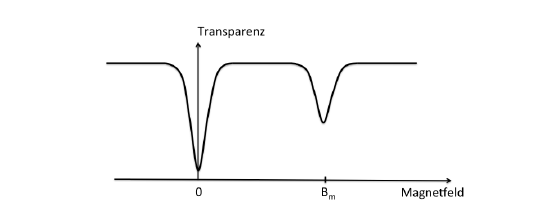
\includegraphics[width=0.8\textwidth]{Resonanz.PNG}
    \caption{Resonanzstellen des Alkali-Atoms in Abhängigkeit vom angelegten Magnetfeld.}
    \label{abb:Resonanz}
\end{figure}
\FloatBarrier

\subsection{Betrachtung für nicht verschwindende Kernspins}
Der nicht verschwindende Kernspin sorgt für weitere Aufspaltungen der Zeeman-Niveaus.
Wird dieses System mit zirkular polarisiertem Licht bestrahlt, so kommt
es lediglich zu Übergängen mit $\Delta \text{M}_{\text{F}} = +1$.
Dies wiederum hat zur Folge, dass lediglich der Zustand $\text{F}=2$ mit $M_F=+2$ besetzt sein wird, da von hier aus kein Übergang mehr induziert werden kann, da kein Niveau mit $\text{M}_{\text{F}}=+3$ existiert und dieser Zustand lediglich durch spontane Emission immer weiter besetzt werden kann.
Somit wird auch hier das Grundniveau "leer gepumpt".

\subsection{Quadratischer Zeeman-Effekt}
Bei stärkeren Magnetfeldern, müssen bei der Berechnung von $E_{\text{HF}}$ Terme höherer Ordnung berücksichtigt werden.
Die Eigenwertgleichung
\begin{align*}
    H \Psi = E \Psi
\end{align*}
wird unter Berücksichtigung der magnetischen Momente $\vec{\mu}_{\text{J}}$ und $\vec{\mu}_{\text{I}}$ und unter Abhängigkeit der Orientierungsquantenzahl $\text{M}_{\text{F}}$ lässt sich dann die Energie wie folgt beschreiben:
\begin{align}
  \label{eq_qZeeman}
    E_{\text{HF}} &= \text{g}_{\text{F}} \mu_{\text{B}} B+ \text{g}_{\text{F}}^2 \mu_{\text{B}}^2 B^2 \frac{1- \text{M}_{\text{F}}}{\Delta E_{\text{Hy}}}- \cdots  \; .
\end{align}
Hierbei ist $E_{\text{Hy}}$ ist die Energiedifferenz der Niveaus F und F$+1$ ist.

\section{Durchführung}
\FloatBarrier
\begin{figure}
    \centering
    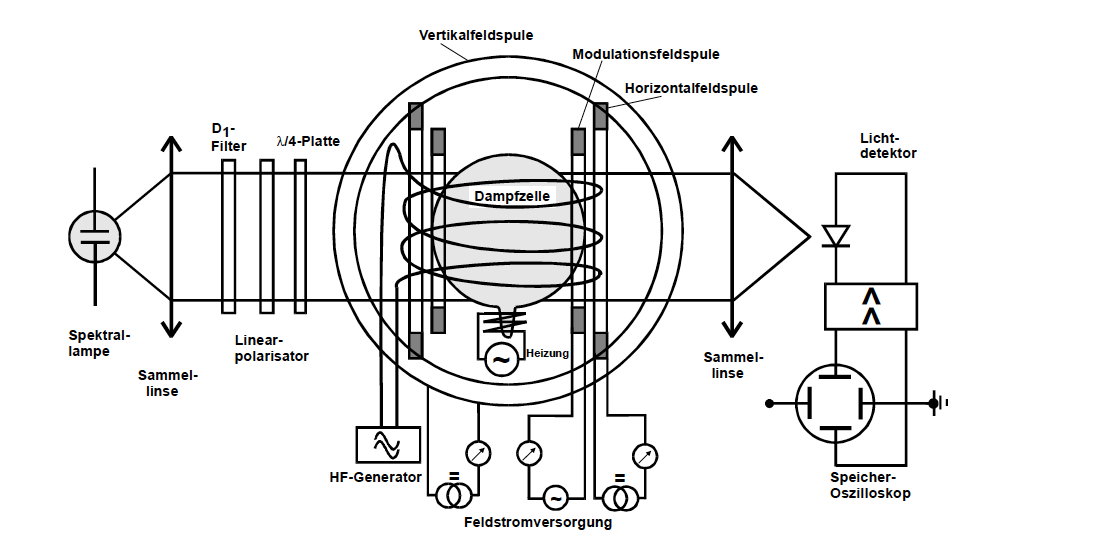
\includegraphics[width=0.9\textwidth]{Aufbau.PNG}
    \caption{schmeatischer Versuchsaufbau}
    \label{abb:Aufbau}
\end{figure}
\FloatBarrier
Der schematische Versuchsaufbau ist in Abbildung \ref{abb:Aufbau} zu sehen.
Zunächst durchläuft das Licht eine Kollimationslinse, die das Licht bündelt. Darauf folgt
ein sogenannter $\text{D}_1$-Filter, der das Licht der Spektrallampe so filtert, dass
lediglich Licht mit einer Wellenlänge von $\lambda = \SI{794,8}{\nano\meter}$ hindurchtritt, was dem Rubidiumspektrum entspricht.
Der Linearpolarisator, der dahinter aufgestellt ist, macht aus dem gebündelten
Lichtstrahl dann zunächst linear polarisiertes Licht, welches dann durch den $\lambda\:/\:4$-Filter zu rechts polarisiertem Licht wird.
Der gebündelte Lichtstrahl durchläuft dann eine Dampfzelle, in der sich $^{85}$Rb
und $^{87}$Rb Isotope als gemisch befinden. Zwischen Dampfzelle und Photodiode befindet
sich abermals eine Sammellinse, um den Lichtstrahl auf den Eingang der Photodiode zu fokussieren. Die Photodiode ihrerseits ist mit einem Oszollospkop verbunden, welches in
Abhängigkeit von der gemessenen Intesität einen Ausschlag in y-Richtung anzeigen wird.

\noindent Um die Zelle herum befinden sich zwei Helmholtzspulenpaare. Eine, um das vertikale Erdmagnetfeld auszugleichen. Um die Spule, die ein horizontales Magnetfeld
erzeugt, ist eine weitere Spule, die Sweep-Spule gewickelt. Diese beiden Spulen werden
benötigt, um die Zeeman-Aufspaltung der Energieniveaus hervorzurufen.
Direkt um die Dampfzelle herum befindet sich eine weitere Spule, die durch einen H
ochfrequenzgenerator mit einer Sinusspannung betrieben wird und somit das RF-Feld
erzeugt. Somit muss nicht die
Energie der einfallenden Photoquanten verändert werden, um Übergänge in den beiden
Rubidiumspektren hervorzurufen, sondern die Übergänge finden in Abhängigkeit zu dem sich ä
ndernden Magnetfeld periodisch statt.
Vor Beginn der Messungen werden zunächst alle optischen Elemente außer der beiden
Kollimationslinsen herausgenommen, um diese so einzustellen, dass eine maximale
Strahlenintensität am Photodetektor ankommt. Ist der Abstand der beiden Linsen
entsprechend justiert, so werden die anderen Elemente in der oben beschriebenen
Reihenfolge eingesetzt.


\subsection{Kompensation des Erdmagnetfeldes}
Da das Erdmagnetfeld einen erheblichen Einfluss auf den Versuchsaufbau hat, muss dieses
ausgegelichen werden. Die horizontale Komponente lässt sich leicht kompensieren, indem
der Versuchsaufbau entlang der Nord-Süd-Achse ausgerichtet wird.
Zur Kompensation der vertikalen Komponente des Erdmagnetfeldes wird das Signal der
Photodiode auf Kanal 2 des Oszilloskops gegeben. Der Recorder-Ausgang der Sweep-Spule
wird auf Kanal 1 gegeben und das Oszilloskop in XY-Betrieb genommen. Im Oszilloskop
stellt sich dann ein breiter, nach unten gerichteter Peak dar, der mit Hilfe der
vertiaklen Spule zu verschmählern ist.

\subsection{Vermessung der Resonanzstellen}
Der Hochfrequenzgenerator des RF-Feldes wird für diesen Veruschsteil von $\SI{100}{\kilo \hertz}$ auf $\SI{1}{\mega \hertz}$ in $\SI{100}{\kilo \hertz}$-Schritten heraufgeregelt.
Zu jeder Frequenz wird das Feld der Horizontalfeldspule so lange heraufgeregelt, bis die
beiden Resonanzstellen im Oszolloskop sichtbar sind. Bei kleineren Frequenzen bis ca.
$\SI{200}{\kilo \hertz}$ reicht das Feld der Sweepspule aus, bei größer werdenden
Frequenzen ist das Feld der Horizontalfeldspule hinzuzunehmen. Die Wertepaare aus
Frequenz und Spulenstrom werden notiert.




\section{Auswertung}

\subsection{Berechnung der Horizontalkomponente des Erdmagnetfelds}
Zur Berechnung des B-Feldes müssen die gemessenen Umdrehungen in einen Strom
$I$ umgerechnet werden, wobei der Umrechnungsfaktor des Sweepfeldes 1 Umdrehung
= \SI{0,1}{\ampere} und der des Horizontalfeldes 1 Umdrehung = \SI{0,3}{\ampere}
beträgt.
Durch die Helmholtzgleichung \eqref{eq:1} kann aus dem Strom $I$ das angelegte
Magnetfeld berechnet werden. Die Messwerte und die daraus berechneten,
überlagerten Magnetfelder sind
in Tabelle \ref{tab:1} zu sehen.
\begin{equation}
  \label{eq:1}
  B = \mu_0 \cdot \frac{8IN}{\sqrt{125}R}
\end{equation}
(Magnetfeld $B$, magnetische Feldkonstante $\mu_0$, Strom $I$, Windungszahl $N$
und Radius $R$)

\begin{table}
  \centering
  \caption{Messwerte und berechnete Magnetfelder}
  \label{tab:1}
  \begin{tabular}{c|ccc}
    \toprule
    $\nu$/\si{\kilo\hertz} & \text{Sweep}/ \text{Umdrehungen} &
    \text{horizontales B-Feld} / \text{Umdrehungen} & $B$/\si{\micro\tesla} \\
    \midrule
    & \multicolumn{3}{l}{1. Isotop} \\
    \midrule
    98,8   &  6,04 &  7,2   & 36,45 \\
    200    &  4,02 &  6,61  & 29,52 \\
    298    &  6,09 &  9,57  & 42,01 \\
    402    &  3,81 &  8,55  & 59,82 \\
    498    &  2,02 &  7,92  & 72,70 \\
    602    &  1,08 &  8,21  & 85,45 \\
    702    &  1,17 &  9,46  & 101,77  \\
    800    &  1,51 &  7,01  & 114,34  \\
    900    &  2,92 &  8,38  & 128,12  \\
    1006   &  5,70 &  7,23  & 144,90  \\
    \midrule
    & \multicolumn{3}{l}{2. Isotop} \\
    \midrule
    98,8  &  7,2   &  0     &  43,45 \\
    200   &  6,61  &  0,02  &  45,15 \\
    298   &  9,57  &  0,02  &  63,01 \\
    402   &  8,55  &  0,14  &  88,43 \\
    498   &  7,92  &  0,23  &  108,31 \\
    602   &  8,21  &  0,30  &  128,47 \\
    702   &  9,46  &  0,36  &  151,80 \\
    800   &  7,01  &  0,49  &  171,22 \\
    900   &  8,38  &  0,55  &  195,27 \\
    1006  &  7,23  &  0,66  &  217,27 \\
    \bottomrule
  \end{tabular}
\end{table}

Zur Berechnung des horizontalen Erdmagnetfeldes wird eine lineare Regression der
Form
\begin{equation*}
  \nu = m \cdot B + b
\end{equation*}
durchgeführt. Bei der Regression wurde jedoch der erste Werte aus der Berechnung
ausgeschlosse, da es eindeutig erkennbar ist, dass dieser falsch gemessen wurde.
Das kann daran liegen, dass wir die Justierschraube auf einer Wert weniger als 0
drehen konnten und es somit nicht ist, ob das B-Feld bei dieser Frequenz vernünftig
eingestellt werden konnte. Deswegen wird der erste Wert bei einer Frequenz von
etwa \SI{100}{\kilo\hertz} in den weiteren Berechnungen vernachlässigt.

Die Steigungen und $y$-Achsenabschnitte sind in Tabelle \ref{tab:2}
aufgelistet. Daraus folgt für das horizontale Erdmagnetfeld
Erdmagnetfeld
\begin{align*}
  B_{\symup{Erde, horizontal, 1}} &= b_1 = \SI{10(10)}{\micro\tesla}\\
  B_{\symup{Erde, horizontal, 2}} &= b_2 = \SI{9(12)}{\micro\tesla}\\
\end{align*}

\begin{table}
  \centering
  \caption{Parameter der Ausgleichsrechnungen}
  \label{tab:2}
  \begin{tabular}{c c c}
    \toprule
    & $m$ / \si{\tesla\second} & $b$ / \si{\tesla} \\
    \midrule
    1. Isotop & \num{1,423(15)e-10} & \num{10(10)e-6} \\
    2. Isotop & \num{2,147(18)e-10} & \num{9(12)e-6} \\
    \bottomrule
  \end{tabular}
\end{table}

\begin{figure}
  \centering
  \includegraphics[scale=0.7]{Bfeld.pdf}
  \caption{Messwerte und lineare Regression.}
  \label{abb:1}
\end{figure}

\subsection{Berechnung der Landéschen Faktoren und des Kernspins}
Die Landéschen Faktoren werden ebenfalls durch die oben berechnete
lineare Regression bestimmt, indem die Regression mit Gleichung \eqref{eq:3}
verglichen wird:
\begin{align*}
  g_{F1} &= \frac{h}{\mu_B m_1} = \num{0,502(5)} \\
  g_{F2} &= \frac{h}{\mu_B m_2} = \num{0,3328(27)} \\
\end{align*}

Zur Berechnung des Kernspins muss zunächst durch Gleichung \eqref{eq:La-Fa.gj}
der Faktor $g_J$ berechnet werden mit $J=S=0,5$, $L=0$ und $g_S = 2,0023$.
Daraus lässt sich dann der Kernspin $I$ mit der Gleichung \eqref{eq:La-Fa.gf}
berechnen:
\begin{align*}
  I_1 &= \num{1,494(21)} \\
  I_2 &= \num{2,508(25)} \\
\end{align*}
Aus dem Vergleich mit den Literaturwerten lässt sich somit eine Verbindung
zu den verwendeten Isotopen herstellen. $^{85}\text{Rb}$ (mit einem Kernspin
$I=5/2$) lässt sich der zweiten Resonanzstelle und $^{87}\text{Rb}$
($I=1/2$) der erste Resonanzstelle zuordnen.

\subsection{Signalbild}
In Abbildung \ref{abb:2} sind die zwei Resonanzstellen eines typischen Signalbildes
zu erkennen.

\begin{figure}
  \centering
  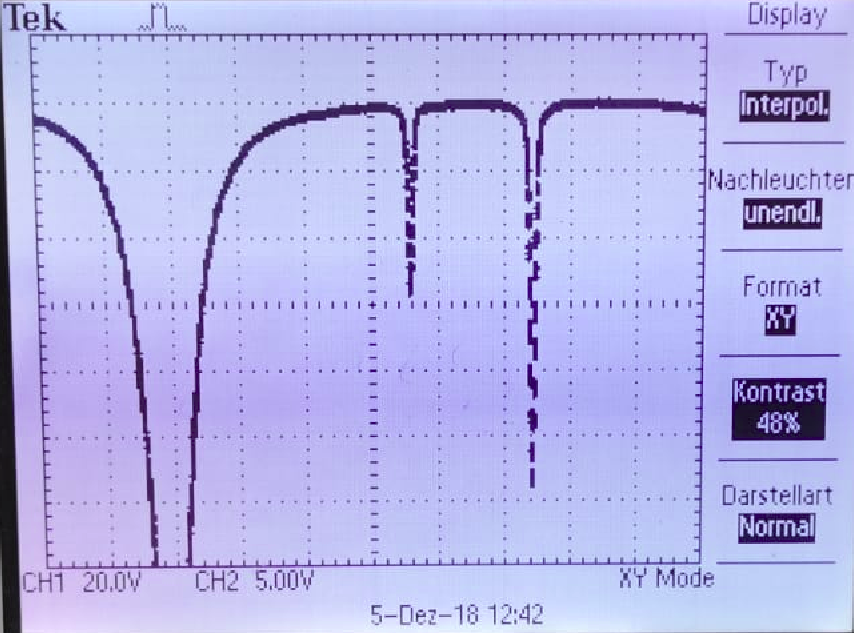
\includegraphics[scale=0.3]{Foto.png}
  \caption{Signalbild mit Resonanzstellen.}
  \label{abb:2}
\end{figure}

Aus dem Amplitudenverhältnis der beiden Resonanzstellen lässt sich auf das
Isotopenverhältnis schließen:
\begin{align*}
  A_1 &= 195\text{px} \\
  A_2 &= 387\text{px} \\
\end{align*}
Damit folgt, dass die Verteilung bei $\approx \SI{33,5}{\percent}$
($^{87}\text{Rb}$) und $\approx \SI{66,5}{\percent}$ ($^{85}\text{Rb}$) liegt.
In der Natur liegen die Isotope in dem
Verhältnis $\approx \SI{72}{\percent}$ ($^{85}\text{Rb}$) und
$\approx \SI{28}{\percent}$ ($^{87}\text{Rb}$) vor.

\subsection{Abschätzung des quadratischen Zeeman-Effekts}
Zur Abschätzung des quadratischen Zeeman-Effekts wird zunächst der lineare Teil
berechnet, um diesen mit dem quadratischen Teil zu vergleichen. Hierbei wird das
maximal gemessene Feld zur Berechnung genommen ( \SI{144,90}{\micro\tesla} und
\SI{217,27}{\tesla} für die jeweiligen Resonanzstellen). Mit $M_F=3$ für
$^{85}\text{Rb}$ und $M_F=2$ für $^{87}\text{Rb}$ und den
Hyperfeinstrukturaufspaltungen \cite{Q1} lässt sich mittels Gleichung \eqref{eq_qZeeman}
die linearen und quadratischen Teile berechnen:
\begin{align*}
  E_{1, linear} &= \SI{4,21(4)e-9}{\eV} \\
  E_{2, linear} &= \SI{4,186(35)e-9}{\eV} \\
  E_{1, quadratisch} &= \SI{-1,88(4)e-12}{\eV} \\
  E_{2, quadratisch} &= \SI{-6,98(12)e-12}{\eV} \\
\end{align*}

\section{Diskussion}
Das horizontale Erdmagnetfeld hat ist in etwa \SI{20}{\micro\meter} groß.
Unsere Messung mit \SI{10(10)}{\micro\tesla} und \SI{9(12)}{\micro\tesla}
liegt jeweils in dem Fehlerintervall, der Fehler ist jedoch sehr hoch.

Der Vergleich der Theoriewerte und der Messwerte des Kernspins zeigen nur sehr
geringe Abweichungen von maximal \SI{0,4}{\percent} und die Theoriewerte liegen
in den Fehlerintervallen der Messwerte (siehe Tabelle \ref{tab:diskussion}).
Daraus zeigt sich, dass dies ein sehr genaues Verfahren zu Messung der
Landéschen Faktoren und des Kernspins ist.

\begin{table}
  \centering
  \caption{Vergleich: Theoriewerte und Messwerte des Kernspins}
  \label{tab:diskussion}
  \begin{tabular}{c| c c c}
    \toprule
    Isotop & Theoriewert & Messwert & Abweichung/\si{\percent}\\
    \midrule
    $^{87}\text{Rb}$ & 1,5 &  \num{1,494(21)} & 0,4 \\
    $^{85}\text{Rb}$ & 2,5 &  \num{2,508(25)} & 0,32 \\
    \bottomrule
  \end{tabular}
\end{table}

Die Verteilung der Isotope ist nicht identisch mir der Verteilung der Isotopen
in der Natur. Dieser weicht um etwa 5,5 Prozentpunkte ab.

Bei der Abschätzung des quadratischen Zeeman-Effektes ist zu erkennen, dass sich
die Werte des linearen und des quadratischen Terms um 3 Größenordnungen
unterscheiden (siehe Tabelle \ref{tab:diskussion2}).
Somit kann davon ausgegangen werden, dass der quadratische
Zeeman-Effekt in diesem Versuch vernachlässigt werden kann.

\begin{table}
  \centering
  \caption{Berechnungen der Energie des quadratischen Zeeman-Effektes.}
  \label{tab:diskussion2}
  \begin{tabular}{c c c}
    \toprule
    Isotop & E linearer Term \si{eV} & E quadratischer Term / \si{\eV} \\
    \midrule
    $^{87}\text{Rb}$ & \num{4,21(4)e-9} & \num{-1,88(4)e-12} \\
    $^{85}\text{Rb}$ & \num{4,186(35)e-9} & \num{-6,98(12)e-12} \\
    \bottomrule
  \end{tabular}
\end{table}
